
\chapter{Revisão Bibliografica}

\section{Veículo omnidirecional de 3 rodas}


\section{Roda Omnidirecional}

A roda omnidirecional aparece em vários modelos na literatura, como exemplo o design feito por J. Graboweicki em 1919 \cite{patent_US1305535A}
o design feito por Josef Blumrich em 1972 \cite{patent_US3789947A}.
A roda consiste em rolos perpendiculares (90°) a direção de giro da roda,o efeito é sua capacidade da roda se mover em mais de uma direção ao mesmo tempo.

\begin{figure}[h]
	\centering
	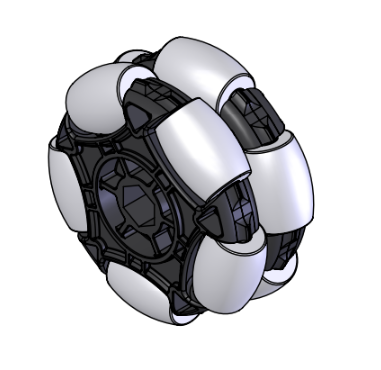
\includegraphics{figures/omniwheel}
	\caption{Modelo de uma Omniwheel \cite{draw_omniwheel}}
\end{figure}

Uma variação da roda omnidirecional é a roda mecanum, inventada por Bengt Ilon \cite{patent_US3876255A}, que possue rolos em 45°.


\section{Microcontrolador STM32F103C8}
O STM32F103C8, também conhecido como Blue Pill, é um microcontrolador fabricado pela STMicroelectronics, de 32-bits, tem como processador o ARM Cortex-M3, de 64Kbs de memória flash.
O processador Cortex-M3, projetado pela ARM (Advanced RISC Machine Ltd.) é  baseado em arquitetura Harvard, de 32-bits.
A família de microcontroladores STM32 fornece uma base par uma uma granda variedades de sistemas embarcados,  e com custo porém essa flexibilidade e custo menor em comparação ao Arduino com o ATmega, que possui microcontroladores de 8 a 16bits.
Porém essa flexibilidade e baixo custo poissui requer um nível de experiência maior em programação C comparado ao Arduino, que foi pensado para ser mais amigável com iniciantes \cite{cortex_m3}.
O STM32F103C8 possui 7 timers, 2 ADCs, e 9 interfaces de comuinicação, incluindo I2C (Inter-Integrated Circuit), USART (Universal Synchronous Asynchronous Receiver Transmitter), SPI (Serial Peripheral Interface), CAN e USB 2.0


\begin{figure}[h]
	\centering
	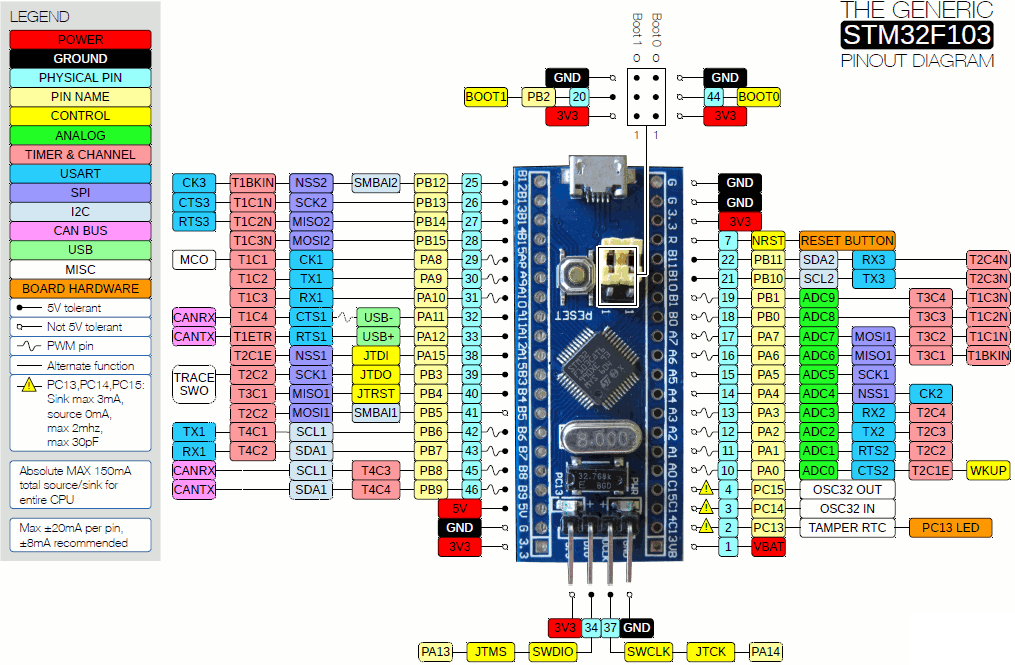
\includegraphics[width=1.0\textwidth]{figures/stm32f1_pinout}
	\caption{Diagrama de pinos do STM32F103C8}
\end{figure}


\section{Motor DC com encoder e driver para motor}

Um motor DC é basicamente uma máquina elétrica de corrente contínua, que converte energia elétrica de corrente contínua em energia mecânica
Máquinas elétricas CC são mais fácies de controlar e oferecem uma grande faixa de velocidades \cite{Maquinas_eletricas}.
Devido a sua facilidade de controle, se tornam ótimos canditados para uso em eletrónica e robótica, pois podem ser usados com baterias
Para controlar a velocidade de um motor, é necessário o uso de um encoder, que converte o sinal de posição em um valor medível de velocidade angular.




cujos aspectos contrutivos são 



